\section{Transformer-XL} \label{sec:TransformerXL}

\subsection{Problem With Transformer} \label{sec:ProblemWithTransformer}


\subsubsection{Fixed-Length Segments} \label{sec:FixedLengthContext}

\nameref{sec:Transformer}s are capable of learning longer term dependencies but instead perform poorer than they should because their inputs are dominated by \textbf{fixed-length context}. Limited context-dependency means that the  largest dependency distance between characters is limited to the input length, which does not allow the \nameref{sec:Transformer} to remember a word that appeared several sentences ago (Dai et al., 2019). 

A \emph{vanilla} (ordinary) \nameref{sec:Transformer} model adapted by Al-Rfou et al. (2018) uses fixed-length context since the model is trained within its segment embeddings. This effectively blocks information from flowing across the segment embeddings during both the \hyperref[sec:ForwardProp]{forward} and \hyperref[sec:BackwardProp]{backward pass}. This result, visible in \cref{fig:transXL_VanillaSegment}, causes the \nameref{sec:Transformer} to forget context from previous segments. 


\begin{figure}[h]
\vspace{-5pt}
\centering
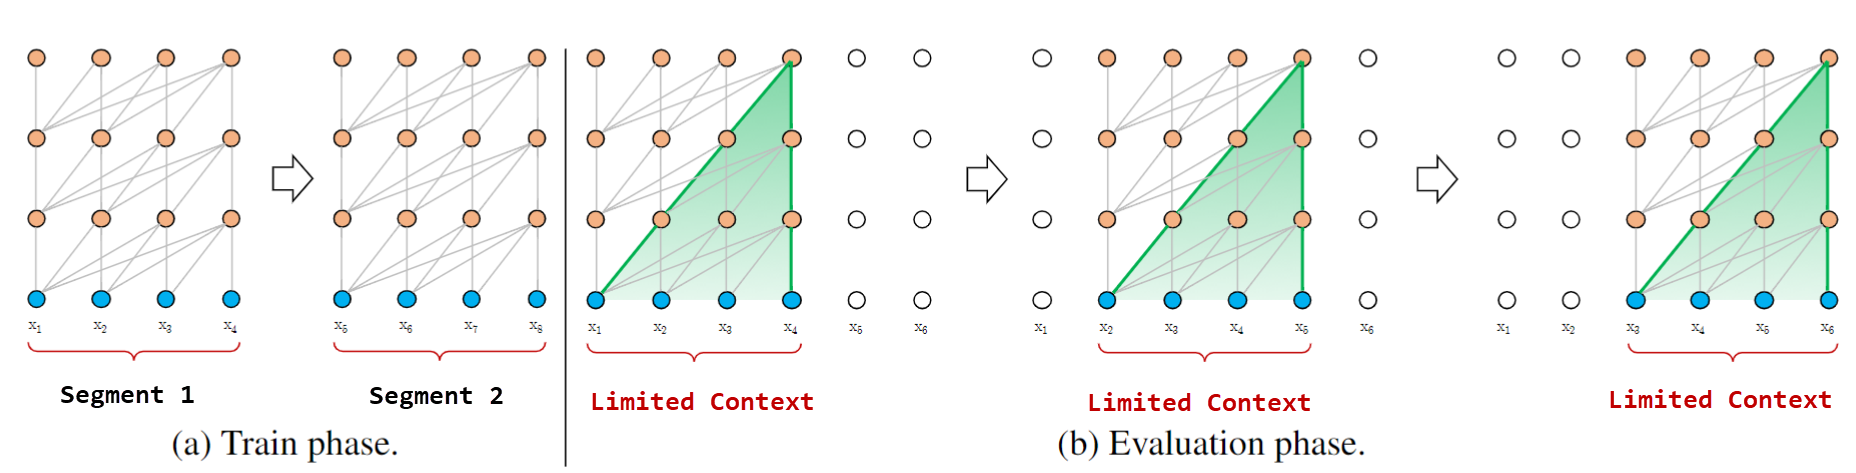
\includegraphics[width=0.99\textwidth]{imgs/transXL_vanillaSegmentation.png}
\vspace{-5pt}
\caption{\footnotesize Vanilla \nameref{sec:Transformer} with segment embedding length $ = 4$. Training the model in fixed-length segments while disregarding natural sentence boundaries results in the \emph{context fragmentation problem}: during each evaluation step, the \nameref{sec:Transformer} consumes a segment embedding and makes a prediction at the last position. Then at the next step, the segment is shifted right by one position only, and the new segment must be processed from scratch, so there is no context dependency for first tokens of each segment and between segments. From \emph{Transformer-XL: Attentive Language Models Beyond a Fixed-Length Context}, by Dai et al., 2019. \url{https://arxiv.org/pdf/1901.02860.pdf}. Copyright 2019 by Dai et al.}
\vspace{-5pt}
\label{fig:transXL_VanillaSegment}
\end{figure}



\subsubsection{Context Fragmentation Problem} \label{sec:ContextFragmentationProblem}

The \nameref{sec:Transformer}'s use of \textbf{fixed-length context} and lack of regard for the natural semantic boundaries of sentences causes it to lose contextual information and perform more poorly than it could. This is called the \textbf{context fragmentation problem}.


\subsection{Motivation for Transformer-XL} \label{sec:MotivationForTransformerXL}

According to Dai et al. (2019), the \textbf{Transformer-XL} (extra long) uses a new architecture that enables learning longer dependencies without ``disrupting temporal coherence." Instead of breaking up sequences into arbitrary \textbf{fixed lengths}, the Transformer-XL \emph{respects natural language boundaries} like sentences and paragraphs, helping it gain richer context over sentences, paragraphs, and even longer texts like documents. It is composed of a \hyperref[sec:SegmentLevelRec]{segment-level recurrence mechanism} and \hyperref[sec:RelativePosEnc]{relative positional encoding} method to resolve \textbf{context fragmentation} and enable representation of longer-spanning dependencies. 


\subsection{Describing Transformer-XL} \label{sec:DescribingTransformerXL}

\subsubsection{Segment-Level Recurrence Mechanism} \label{sec:SegmentLevelRec}

To resolve \textbf{context fragmentation}, the Transformer-XL employs a \textbf{segment-level recurrence mechanism} to capture long-term dependencies using information from previous segments. While intaking the first segment of tokens like the vanilla \nameref{sec:Transformer}, this new recurrence mechanism also stores hidden layer outputs. This is so that when a segment is being processed, each hidden layer receives two inputs: (1) the previous hidden layer outputs of the \emph{current segment} (as the vanilla model, shown as gray arrows in \cref{fig:transXL_extendedContext}), and (2) the previous hidden layer outputs of the \emph{previous segment} (green arrows in \cref{fig:transXL_extendedContext}). These features build long-term memory (Horev, 2019). 

\begin{figure}[h]
\vspace{-5pt}
\centering
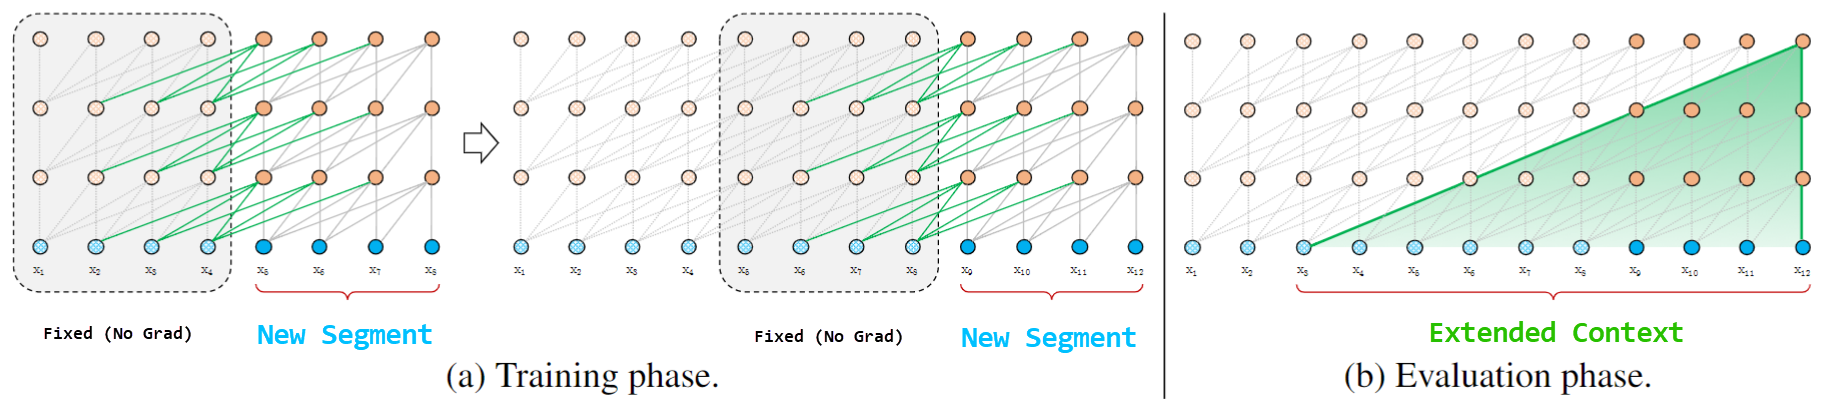
\includegraphics[width=0.99\textwidth]{imgs/transXL_extendedcontext.png}
\vspace{-5pt}
\caption{\footnotesize Segment level recurrence mechanism at work: the hidden state for previous segment is \emph{fixed} and \emph{stored} to later be reused as an extended context while the new segment is processed. Like in \nameref{sec:Transformer}, gradient updates or training still occurs within a segment, but the extended context feature allows historical information to now be incorporated. From \emph{Transformer-XL: Attentive Language Models Beyond a Fixed-Length Context}, by Dai et al., 2019. \url{https://arxiv.org/pdf/1901.02860.pdf}. Copyright 2019 by Dai et al.}
\vspace{-5pt}
\label{fig:transXL_extendedContext}
\end{figure}

Although gradient updates or training still occurs within a segment, the extended context feature allows historical information to be fully used, avoiding context fragmentation. 

Intuitively, for the sentence ``I went to the store. I bought some cookies," the model receives the sentence ``I went to the store," caches the hidden states, and only \emph{then} feeds the other part ``I bought some cookies" with the cached states into the model (Kurita, 2019b). 

Formally, the recurrence mechanism is described as follows. Let $\textbf{s}_\tau = \Big\{ x_{\tau_1}, x_{\tau_2}, ..., x_{\tau_L} \Big\}$ and $\textbf{s}_{\tau + 1} = \Big\{ x_{{\tau+1}_1}, x_{{\tau+1}_2}, ..., x_{{\tau+1}_L} \Big\}$ denote two consecutive segment embeddings of length $L$. Let $\textbf{h}_\tau^n \in \mathbb{R}^{L \times d}$ be the $n$-th layer's hidden state vector produced for the $\tau$-th segment $\textbf{s}_\tau$, where $d$ is the hidden dimension. Then the $n$-th layer's hidden state for next segment $\textbf{s}_{\tau + 1}$ is calculated as:
$$
\begin{array}{ll}
\large \Tilde{\textbf{h}}_{\tau + 1}^{n-1} = \Big\{ \textit{StopGradient}\Big( \textbf{h}_\tau^{n-1} \circ \textbf{h}_{\tau+1}^{n-1} \Big) \Big\} \\\\
%
\large \textbf{q}_{\tau+1}^n, \;\;\; \textbf{k}_{\tau+1}^n, \;\;\; \textbf{v}_{\tau+1}^n = \textbf{h}_{\tau+1}^{n-1} \cdot \textbf{W}_q^T, \;\;\; \Tilde{\textbf{h}}_{\tau+1}^{n-1} \cdot \textbf{W}_k^T, \;\;\; \Tilde{\textbf{h}}_{\tau+1}^{n-1} \cdot \textbf{W}_v^T \\\\
%
\large \textbf{h}_{\tau+1}^n = \textit{TransformerLayer} \Big( \textbf{q}_{\tau+1}^n, \;\;\; \textbf{k}_{\tau+1}^n \;\;\; \textbf{v}_{\tau+1}^n \Big)
\end{array}
$$
where the first line indicates that the two consecutive hidden states are concatenated; $\textbf{W}$ denotes model parameters; and $\textbf{q}, \textbf{k}, \textbf{v}$ are the \hyperref[sec:QKV]{query, key, and value vectors}. The key feature here, compared to standard \nameref{sec:Transformer}, is that the key $\textbf{k}_{\tau+1}^n$ and value $\textbf{v}_{\tau+1}^n$ are conditioned on the elongated context $\Tilde{\textbf{h}}_{\tau+1}^{n-1}$ \emph{and} the previous segment's cached context $\textbf{h}_\tau^{n-1}$. This is visible by the green lines in \cref{fig:transXL_extendedContext}.  

This new recurrence scheme allows more efficient computations. Also, it can cache multiple previous segments not just the previous one, making it more similar to an \hyperref[sec:RNN]{RNN's memory}. 


\subsubsection{Relative Positional Encoding} \label{sec:RelativePosEnc}

Introducing the \hyperref[sec:SegmentLevelRec]{segment-level recurrence mechanism} presented a problem: how can positional word order be kept coherent when reusing hidden states? The vanilla \nameref{sec:Transformer} kept word order straight using \hyperref[sec:PosEncodings]{positional encodings}. But since the standard \nameref{sec:Transformer}'s \hyperref[sec:PosEncodings]{positional encodings} are based on \emph{absolute distance} between tokens, applying these directly to the Transformer-XL caused consecutive word embedding sequences to be associated with the same \hyperref[sec:PosEncodings]{positional encoding}, so the model could not distinguish the difference in positions of consecutive input tokens. This means that tokens from different segments had the same \hyperref[sec:PosEncodings]{positional encodings}, even though their position and importance could differ. This confused the model. 

To remedy this and make their recurrence scheme work, the authors created a \textbf{relative \hyperref[sec:PosEncodings]{positional encoding}} scheme that works in conjunction with each \hyperref[sec:AttentionMechanism]{attention score} of each layer, rather than encoding position only before the first layer, and which is based on \emph{relative} distance between tokens, not \emph{absolute} position (Horev, 2019). Formally, the authors created a relative \hyperref[sec:PosEncodings]{positional encoding}s matrix whose $i$-th row indicates a relative distance of $i$ between two positions, and injected this dynamically into the attention module. This lets the query vector now distinguish between two tokens from their different distances. Now, from Dai et al. and Horev (2019), the attention head calculation has four parts: 
\begin{enumerate}
    \item \textbf{Content-based addressing: }the original attention score without \hyperref[sec:PosEncodings]{positional encoding}.
    
    \item \textbf{Content-dependent positional bias: }with respect to the current query. It uses a sinusoidal function that get distance between tokens instead of the \emph{absolute position} of a single current token. 
    
    \item \textbf{Learned global content bias: } is a learned vector that accounts for the other tokens in the key matrix.
    
    \item \textbf{Learned global positional bias: }is a learned vector that adjusts the importance based only on distance between tokens, using the intuition that recent previous words are more relevant that a word from the previous paragraph. 
\end{enumerate}


\subsection{Experimental Results of Transformer-XL} \label{sec:ExpResultsTransXL}

\subsubsection{Ablation Study for Segment-Level Recurrence and Relative Positional Encodings}

The authors seek to isolate the effects of Transformer-XL's \hyperref[sec:SegmentLevelRec]{segment-level recurrence mechanism} using with different encoding schemes. In \cref{tbl:transXL_ablationRECURR}, Shaw et al. (2018) uses relative encodings, and Vaswani and Al-Rfou use absolute encodings. 






\begin{figure}[h]
\vspace{-5pt}
\centering
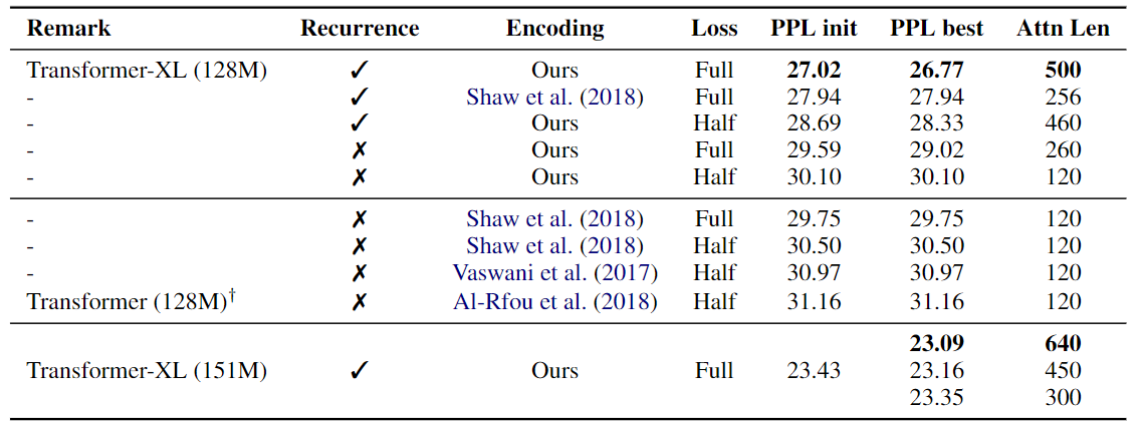
\includegraphics[width=0.99\textwidth]{imgs/table_transXL_ablationREC.png}
\vspace{-5pt}
\captionof{table}{\footnotesize Ablation study for \nameref{sec:SegmentLevelRec} on the WikiText-103 data set. \textbf{PPL best} (model output) means perplexity score obtained using an optimal \hyperref[sec:BackwardProp]{backpropagation} training time length. \textbf{Attn Len} (model input) is the shortest possible attention length during evaluation to achieve the corresponding PPL best. From \emph{Transformer-XL: Attentive Language Models Beyond a Fixed-Length Context}, by Dai et al., 2019. \url{https://arxiv.org/pdf/1901.02860.pdf}. Copyright 2019 by Dai et al.}
\vspace{-5pt}
\label{tbl:transXL_ablationRECURR}
\end{figure}


The \cref{tbl:transXL_ablationRECURR} shows that both \hyperref[sec:SegmentLevelRec]{segment-level recurrence} and the \hyperref[sec:RelativePosEnc]{relative positional encoding} must be used in conjunction for best performance, since when using the new recurrence with the new encodings, the Transformer-XL can generalize to larger attention sequences (with length $500$) during evaluation while getting lowest perplexity score of $26.7$. However, if the Transformer-XL does not use the new recurrence and uses the new encodings, even using shorter attention sequences of $260$ and $120$ with different \hyperref[sec:BackwardProp]{backprop} loss schemes cannot help lower its perplexity scores, as shown in the last two rows of \cref{tbl:transXL_ablationRECURR}'s Transformer-XL section. The standard \nameref{sec:Transformer} does poorly in general, showing high overall perplexities even using short attention lengths. 
